\documentclass[conference]{IEEEtran}
\usepackage{cite}
\usepackage{amsmath,amssymb,amsfonts}
\usepackage{algorithmic}
\usepackage{graphicx}
\usepackage{textcomp}
\usepackage{xcolor}
\graphicspath{{sources/}}
\def\BibTeX{{\rm B\kern-.05em{\sc i\kern-.025em b}\kern-.08em
    T\kern-.1667em\lower.7ex\hbox{E}\kern-.125emX}}
\begin{document}

\title{Apache Spark GraphX vs Apache Flink: A Graph Processing Performance Comparison\\
}

\author{\IEEEauthorblockN{Georgios Kyriakopoulos}
\IEEEauthorblockA{\textit{School of Electrical and Computer Engineering} \\
\textit{National Technical University of Athens}\\
Athens, Greece \\
el18153@mail.ntua.gr}
\and
\IEEEauthorblockN{Serafeim Tzelepis}
\IEEEauthorblockA{\textit{School of Electrical and Computer Engineering} \\
\textit{National Technical University of Athens}\\
Athens, Greece \\
el18849@mail.ntua.gr}
}

\maketitle

\begin{abstract}
The goal of this paper is to develop a system that allows for the comparison of the performance of graph processing systems. The comparison is based on the same dataset, workload, and hardware environment, and the results are validated. The system executes predefined queries on each system under test, measures the time required to complete each task, computes performance metrics for each system, and produces graphical representations of each metric for each SUT. The functions that are compared include finding the shortest path, degree centrality, triangle count, and weakly connected components. The two systems compared are Apache Spark GraphX and Apache Flink. Performance metrics include average, minimum and maximum query execution time.
\end{abstract}

\begin{IEEEkeywords}
performance comparison, graph processing, benchmarking, execution time, shortest path, degree centrality, triangle count, weakly connected components, Apache Spark GraphX, Apache Flink
\end{IEEEkeywords}

\section{\textbf{Introduction}}\label{intro}
The rise of big data, characterized by large and complex datasets generated by various sources, including social media, sensors, and other digital technologies, has led to the emergence of new tools and approaches for managing and analyzing data. Graph processing systems have become increasingly popular as a way to analyze large-scale graph datasets and extract valuable insights and patterns.

However, with a wide range of available graph processing systems, selecting the most suitable one for a given use case can be a challenging task. Furthermore, comparing the performance of these systems is a complex and time-consuming process that requires a standardized methodology and set of metrics to ensure fair and accurate comparisons. Therefore, the goal of this project is to develop a system that allows for the comparison of two popular graph processing systems, Apache Spark GraphX \cite{b1} and Apache Flink \cite{b2}, under the same conditions.

The primary objective of this project is to compare the performance of these systems using a standardized set of graph processing queries, including finding the shortest path, degree centrality, triangle count, and weakly connected components. By comparing these systems, we aim to identify their respective strengths and weaknesses and provide insights into their potential use cases.

To achieve this goal, we will implement a system that can execute predefined queries on each system under test, measure the time required to complete each task, compute performance metrics, and produce graphical representations of each metric for each SUT. The system will be designed to ensure that the comparison is fair, using the same dataset, workload, and hardware environment for each system under test. The results will be validated to ensure their accuracy and reliability.

The rest of this paper is organized as follows:

\begin{itemize}
\item Section \ref{data}: Dataset
\item Section \ref{sut}: System Under Test Setup
\item Section \ref{graphx}: Apache Spark GraphX
\item Section \ref{flink}: Apache Flink
\item Section \ref{outs}: Outputs Analysis
\item Section \ref{times}: Execution Runtimes Analysis
\item Section \ref{final}: Conclusion
\end{itemize}

This paper is backed by a GitHub repository \cite{b3} \cite{b4}, which contains the source code of the system, the dataset, and the results of the comparison, as well as analytics for the outcomes.

\section{\textbf{Dataset}}\label{data}
The choice of the dataset is a critical aspect of performance comparison in graph processing systems. A well-selected dataset should be representative of real-world scenarios, sufficiently large, and diverse enough to challenge the capabilities of the systems under test. In this section, we describe the dataset selected for our comparison and its characteristics.

We have chosen the Google web graph dataset \cite{b5} \cite{b6}. It is an interesting and widely used dataset in the field of graph processing. It represents the structure of the World Wide Web, where nodes represent web pages and edges represent hyperlinks between them. The graph is directed, and the edges represent the hyperlink relationship from one page to another.

The Google web graph dataset is challenging to process due to its size and complexity, with 875,713 nodes and 5,105,039 edges. However, it is an excellent choice for performance comparison in graph processing systems as it represents a real-world scenario and can be used to test the scalability and efficiency of the systems under test.

The Google web graph dataset is publicly available, after being released in 2002 by Google, as a part of the Google Programming Contest. It has been used in various research studies, which makes it a suitable choice for our comparison. By using this dataset, we aim to provide insights into the performance of Apache Spark GraphX and Apache Flink in processing large-scale web graphs and identifying their respective strengths and weaknesses.

The dataset was downloaded from the Stanford Network Analysis Platform \cite{b5}, which is a collection of large-scale datasets that are used for research in graph processing and data mining. The dataset consisted of only one file, named web-Google.txt, that included the edges of the network as pairs of source and target vertices. The dataset was 72MB in size.

Additionally, there are several statistics associated with the Google web graph dataset that will be discussed in the output validation section. These statistics include degree distribution, number of nodes in the largest weakly connected component, triangle count, etc.

After testing several larger datasets, we ultimately chose the Google web graph dataset as it was within the computational limits of our resources. This choice was made after careful consideration of the other datasets we tested and their resource requirements. Overall, the Google web graph dataset was deemed suitable for our research needs and the available resources.

It is important to acknowledge that the performance of the systems under test may vary with larger datasets, and additional testing may be required to determine their scalability and performance with even larger graphs. However, we believe that the Google web graph dataset provides a good representation of a large-scale graph that is challenging to process and allows for a fair comparison between Apache Spark GraphX and Apache Flink.

\section{\textbf{System Under Test Setup}}\label{sut}

\subsection{Virtual Machines and cluster}

In this section, we outline the procedures that were used to acquire the virtual machines for our systems and to set up our multi-node cluster.

We used the okeanos IAAS \cite{b7}, which is GRNET's cloud service, for the Greek Research and Academic Community, to acquire 3 virtual machines for our study. Each machine has the same following specifications:

\begin{itemize}
\item CPU: 4 Cores - Intel\textregistered\ Xeon\textregistered\ CPU E5-2650 v3
\item RAM: 8GB
\item Disk: 30GB
\item Operating System: Ubuntu Server 16.04.3 LTS
\end{itemize}

Those 3 machines were used to set up a multi-node cluster consisting of one master node and 2 worker nodes.

As for networking, we were given one public IPv4, which we tied to our master machine. Then, we also set up a local network (192.168.1.0/24) so that the 3 nodes could communicate with each other, where 192.168.1.1 was assigned to the master node and 192.168.1.2 and 192.168.1.3 to the 2 worker nodes.

\subsection{Initial Configuration}

After setting up our machines, we used SSH in order to connect and have access to them and proceed with the configuration.

First of all, we changed the hostnames of our machines to master, slave1 and slave2 respectively and also added all the private IPv4 addresses of the local network to the /etc/hosts file, along with the hostnames, for every node.

To avoid possible mistakes and for easier and quicker configuration of our machines, we utilized some bash scripts. The first of those generated an SSH key pair (public and private) on the master node, using the RSA algorithm, and used it to set up passwordless ssh between the master and the worker nodes.

The second script was for setting up a NAT. The use of a NAT allows a single public IP address to be shared among many devices on a local network. In our case, only the master node had a public IPv4 and could access the internet. Therefore, we added the master node’s IPv4 as a default gateway to the worker nodes, after we had enabled IPv4 forwarding on it and set it up to operate as a router.

\subsection{Software Installation}

The first step was to install the Java Development Kit (JDK) \cite{b8}, using a script, on all 3 nodes. We chose version 1.8 which was compatible with both Apache Spark and Flink. 

After that, we could proceed with the installation of Apache Spark \cite{b9}. The script we used downloaded and configured Spark in the same way for all 3 nodes. We chose version 3.3.1, which was the latest stable version at the time of our study. As for configuration, we set the master node as the Spark master, running at port 7077 and the 2 worker nodes, as well as the master node, as Spark workers. Every worker had 2 executor cores and 3g memory per executor. The driver memory was set to 512m. Those selections were made based on the specifications of our machines and the dual role of the master node as both the Spark master and a Spark worker.

GraphX comes with Apache Spark, so we did not need to install it separately. However, in order to write and compile the queries, using Scala, as our preference, we had to install Scala \cite{b10} and the Scala Build Tool (SBT) \cite{b11}. That was only necessary for the master node, as we were compiling and submitting our jobs there. The version of Scala we used was 2.11.6 and the version of SBT was 1.8.2.

We then had to install and configure Apache Flink. We chose version 1.16.1, which was the latest stable version at the time of our study. We installed Flink on all 3 nodes and set the master node as the Flink JobManager. The 2 worker nodes and the master node were set as Flink TaskManagers. The master node was also used to run the JobManager Web UI, running at port 8081. For memory, JobManager had 2g total available, while TaskManagers had 7g. We also used 2 task slots per TaskManager and set the parallelism to 6, equalling the total number of tasks available. Those selections were made based on the specifications of our machines and the dual role of the master node as both the Flink master and a Flink worker.

Having set up Flink, we had to install Maven \cite{b12} in order to compile and run the Java jobs that we wrote for Flink. We used version 3.3.9. On a similar note with the Scala and SBT installation, we only needed to install Maven on the master node, as we were compiling and submitting our jobs there.

\subsection{Dataset}

We downloaded the web-Google dataset from the Stanford Network Analysis Platform \cite{b5}, in a compressed gzip format on our master node. After unzipping it, we moved it to a data folder and copied it to the worker nodes as well so that every node would have access to it.

\section{\textbf{Apache Spark GraphX}}\label{graphx}

\subsection{Introduction}

Apache Spark GraphX \cite{b1} is a distributed graph processing system that is built on top of the popular Apache Spark framework. GraphX provides a unified programming model for graph computation and allows for the efficient processing of large-scale graphs.

GraphX works by representing a graph as a collection of vertices and edges, where vertices represent the nodes of the graph, and edges represent the relationships between nodes. GraphX uses the Resilient Distributed Dataset (RDD) abstraction of Spark to store and manipulate graph data. It utilizes the vertex-centric programming model, which allows users to express graph algorithms as a set of message-passing operations between vertices and their neighbors

GraphX provides a set of graph operators and functions that can be used to perform various graph computations, such as shortest path, degree centrality, triangle count, and weakly connected components. These operators and functions are optimized for distributed processing, allowing for efficient computation of large-scale graphs across a cluster of machines, since the library is designed to work with graphs that are too large to fit into the memory of a single machine, enabling it to distribute graph computation to achieve high performance and scalability.

After this brief explanation of how GraphX works, we can proceed with the general query procedure we followed and with an analysis of each one of the operations implemented for our study.

For all the queries, we followed a similar approach and structure. First, we created a \verb|SparkSession| object, which is the entry point to Spark functionality and set the Spark \verb|master| and \verb|AppName|. Then, we loaded the dataset from the local \verb|web-Google.txt| edge list file into a Graph object, using the \verb|GraphLoader.edgeListFile| function. After that, we executed the operation that was needed on the graph to receive the desired output. Finally, we saved the results of the query into a local text file, using the \verb|FileWriter| and \verb|BufferedWriter| objects and stopped the Spark context.

\subsection{Degree Centrality}

To compute the Degree Centrality of our dataset graph, we used the \verb|degrees| function of the \verb|org.apache.spark.graphx| module. This function returns a \verb|VertexRDD| object, which is a distributed collection of key-value pairs, where the key is the vertex ID and the value is the degree of the vertex. We then used a map function to change the format of the output to \verb|vertexID degree|, so that it would be easier to read and understand.

\subsection{Shortest Paths}

To compute the Single Source Shortest Paths of our dataset graph, we used the \verb|ShortestPaths| function from the \verb|org.apache.spark.graphx.lib| module. This function takes a Graph and a list of landmark vertices as arguments and returns a Graph where each vertex attribute is a map containing the shortest-path distance to each reachable landmark vertex. Since we wanted to calculate the Single Source Shortest Paths, we first created a \verb|reversedEdges| object, where we reversed the direction of the edges of the graph and then created a \verb|reversedGraph| Graph with the same vertices as the original graph and the \verb|reversedEdges| as its edges. Then, we used the \verb|ShortestPaths| function to calculate the shortest paths from the source vertex with ID equal to 0. Finally, we used a \verb|map| function to change the format of the output to \verb|vertexID shortestPath|.

\subsection{Triangle Count}

To compute the Triangle Count of our dataset graph, we used the \verb|TriangleCount| function from the \verb|org.apache.spark.graphx.lib| module. This function takes a Graph as an argument and returns a Graph where each vertex attribute is the count of triangles that include that vertex. Then, we used a \verb|map-reduce| function where we kept just the triangle counts of all the vertices, added them all together and divided by 3 to get the total number of triangles in the graph, since every triangle was counted 3 times, one for each of the 3 different vertices in it. This time we did not need to change the format of the output, since it was just one count and already in the desired format.

\subsection{Weakly Connected Components}

To compute the Weakly Connected Components of our dataset graph, we used the \verb|ConnectedComponents| function from the \verb|org.apache.spark.graphx.lib| module. This function takes a Graph as an argument and returns a Graph where each vertex attribute is the lowest vertex ID in the weakly connected component containing that vertex. Then, we used a \verb|map| function to change the format of the output to \verb|vertexID componentID|.

\subsection{Building and Submitting a Job}

To initialize the Scala project for the GraphX queries, we used the \verb|sbt new scala/scala-seed.g8| command. This command creates a new sbt project and receives the name of the project as input. Then, we added the \verb|org.apache.spark %% spark-core % 3.3.1| and \verb|org.apache.spark %% spark-graphx % 3.3.1| library dependencies to the \verb|build.sbt| file. After that, we created a new file for each query named after the query, under \verb|<project-dir>/src/main/scala/|.

Then, we used the \verb|sbt package| command to compile the project and create a jar file that we could submit to the Spark cluster. Before submitting the job, we had to start the Spark cluster by running the \verb|start-all.sh| script on the master node. To submit a job, we used the \verb|spark-submit| command, which receives the class name to be executed as an argument, using \verb|--class <class-name>|, as well as the path to the jar file. It was then possible to monitor the progress of the job using the Spark UI, which was available at \verb|http://<master-public-ip>:8080|.

\section{\textbf{Apache Flink}}\label{flink}

\subsection{Introduction}

Apache Flink \cite{b2} is an open-source, distributed computing system that is designed to process large-scale data in a fault-tolerant and efficient manner. It is a powerful tool for processing and analyzing large graph datasets and offers several features and optimizations that make it an attractive option for graph processing tasks.

One of the key advantages of Apache Flink for graph processing is its support for iterative processing. In many graph algorithms, such as the PageRank algorithm, the same operation must be performed repeatedly until a convergence criterion is met. Apache Flink offers built-in support for iterative processing, which can significantly reduce the execution time and improve the efficiency of these algorithms.

Additionally, Apache Flink provides a variety of graph processing APIs, including Gelly, which make it easy to write and execute graph algorithms. This API offers a range of graph processing functions, such as vertex-centric iteration, graph partitioning, and graph filtering, which can be used to implement a wide range of graph processing tasks, such as shortest path, degree centrality, triangle count, and weakly connected components. These operators and functions are optimized for distributed processing, allowing for efficient computation of large-scale graphs across a cluster of machines.

The same methodology and structure was used for all the queries, as was the case with GraphX. First, we set up the \verb|ExecutionEnvironment| object, which is the entry point to our Flink application. Then, we loaded the dataset from the local \verb|web-Google.txt| edge list file into a \verb|DataSet| of \verb|Tuple2<Integer, Integer>|, using the \verb|env.readTextFile| function. Afterwards, we created the Graph object from the \verb|DataSet| of tuples, using the \verb|Graph.fromTuple2DataSet| function. Next, we executed the operation that was needed on the graph to receive the desired output. Finally, we saved the results of the query into a local text file, using the \verb|FileWriter| and \verb|BufferedWriter| objects.

\subsection{Degree Centrality}

To compute the Degree Centrality of our dataset graph, we used the function \verb|getDegrees| from the \verb|org.apache.flink.graph.Graph| module. This function returns a \verb|DataSet| of \verb|Tuple2<Integer, LongValue>|, where the first element of the tuple is the vertex ID and the second element is the degree centrality of the vertex. We then added each tuple on an \verb|ArrayList| that was later used to print the output in a format of \verb|vertexID degree|.

\subsection{Shortest Paths}

To compute the Single Source Shortest Paths of our dataset graph, we used the \verb|SingleSourceShortestPaths| from the \verb|org.apache.flink.graph.library| module. This function takes a weighted Graph as an argument and returns a \verb|DataSet| of \verb|Vertex<Integer, Double>|, where the first element of the tuple is the vertex ID and the second element is the shortest path distance from the source vertex. To construct the weighted Graph we used a \verb|map| function to add a default weight of 1.0 to each edge of the graph and then constructed the new weighted Graph based on the weighted edges. Then, in order to use the \verb|SingleSourceShortestPaths| function to calculate the shortest paths from the source vertex with ID equal to 0, we first created a new instance of it, passing the source vertex ID and the maximum iterations as arguments. We used maximum iterations equal to 100, which is big enough to allow the algorithm to converge before reaching the number of maximum iterations, and run the algorithm. Finally, we added every vertex with its vertex value to an \verb|ArrayList| that was later used to print the output in a format of \verb|vertexID shortestPath|.

\subsection{Triangle Count}

To compute the Triangle Count of our dataset graph, we used the \verb|TriangleEnumerator| function from the \verb|org.apache.flink.graph.library| module. This function returns a \verb|DataSet| of \verb|Tuple3<Integer, Integer, Integer>|, where each tuple represents a unique triangle in the graph and each of the elements is a vertex participating in the triangle. We then counted the number of tuples in the \verb|DataSet| to get the total number of triangles in the graph. This time we did not need to change the format of the output, since it was just one count and already in the desired format.

\subsection{Weakly Connected Components}

To compute the Weakly Connected Components of our dataset graph, we used the \verb|ConnectedComponents| function from the \verb|org.apache.flink.graph.library| module. This function takes a Graph with vertex values as an argument and returns a \verb|DataSet| of \verb|Vertex<Integer, Integer>|, where the first element of the tuple is the vertex ID and the second element is the lowest vertex ID in the weakly connected component containing that vertex. To construct the graph with vertex values, we annotated our Graph using a \verb|map| function, where every vertex got its ID as a vertex value. Then, in order to use the \verb|ConnectedComponents| function to calculate the weakly connected components, we first created a new instance of it, passing the maximum iterations as an argument. We used maximum iterations equal to 100, with a similar goal, as in the shortest Paths case, to allow the convergence of the algorithm, and then run the algorithm. Finally, we added every vertex with its vertex value to an \verb|ArrayList| that was later used to print the output in a format of \verb|vertexID componentID|.

\subsection{Building and Submitting a Job}

The initialization of a project for a Flink Java Job was done through \verb|mvn archetype:generate|. This command creates a new maven project and receives the group, name, version and packaging as input. Then, a few changes to the \verb|pom.xml| file were made, such as the name of the job, the name of the \verb|mainClass| and the Flink Gelly dependency was added on the dependencies section. After that, we renamed the main java file and its main class to the name of the job.

Then, we used the \verb|mvn clean package| command to compile the project and create a jar file that we could submit to the Flink cluster. Before submitting the job, we had to start the Flink cluster by running the \verb|start-cluster.sh| script on the master node. To submit a job, we used the \verb|flink run| command, which receives the path to the jar file as an argument. It was then possible to monitor the progress of the job using the Flink UI, which was available at \verb|http://<master-public-ip>:8081|.

\section{\textbf{Outputs Analysis}}\label{outs}

In the following section we will first cross validate that the two libraries produce the same outputs for the queries on our dataset and then perform some analysis on their outputs and validate them against given statistics. We will base our method on the outputs Jupyter Notebook \cite{b13} found in the GitHub repository of the project under the analytics directory \cite{b3} \cite{b4}.

Both this notebook and the times one that we will use to present the execution times in the next section were run on Google Colab \cite{b14}, which is a free Jupyter notebook environment that requires no setup and runs entirely in the cloud, and the outputs and times files were uploaded on its platform.

\subsection{Cross Validation}

We first had to make sure that both libraries produce the same outputs for the queries on our dataset. To do that, we loaded the outputs of the queries from the outputs files that were generated by the two libraries for all the queries that we run. We then checked to make sure that every output was the same for both libraries by checking the outputs one by one.

All of the queries produced the same outputs for both libraries, which means that the two libraries are cross validated and we can move on to the analysis part for each query.

\subsection{Degree Centrality}

We calculated the maximum degree and the average degree of our graph, using a pandas dataframe \cite{b15} and iterating the degrees column of the outputs of the degree centrality query. The maximum degree was found to be 6353 and the average degree 11.6592. These are in accordance with the values Maximum degree and Average degree on the dataset statistics \cite{b6}.

We also plotted the Degree Centrality Distribution log Plot of our graph. The plot is shown in Figure \ref{degreePlot}. The distribution of the degree centrality values is a power law distribution, meaning there are a lot of vertices with low degree centrality and a few vertices with high degree centrality. This is in accordance with the Degree Distribution plot on the dataset plots \cite{b6}.

\begin{figure}[htbp]
\centerline{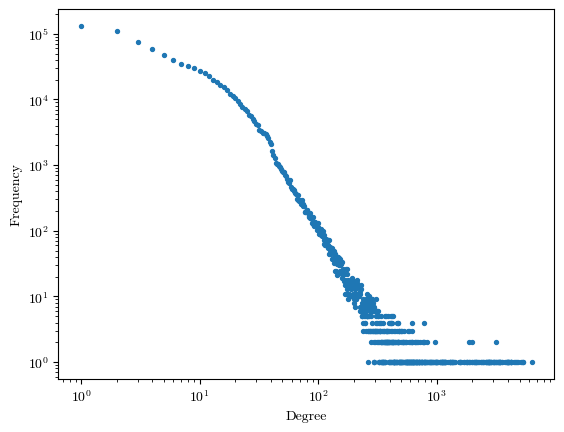
\includegraphics[width=0.5\textwidth]{degree-centrality-distribution.png}}
\caption{Degree Centrality Distribution log Plot}
\label{degreePlot}
\end{figure}

\subsection{Shortest Paths}

The calculation of the maximum and the average shortest path distance was executed, using a pandas dataframe \cite{b15} to filter the infinite values out. The maximum shortest path distance was found to be 32 and the average shortest path distance 11.2628.

Also the Shortest Paths Distribution Plot was produced, as shown in Figure \ref{sPathsPlot}. The distribution of the shortest path distances is a Poisson distribution around the average shortest path distance. However, no other statistics are available for the shortest paths to validate against.

\begin{figure}[htbp]
\centerline{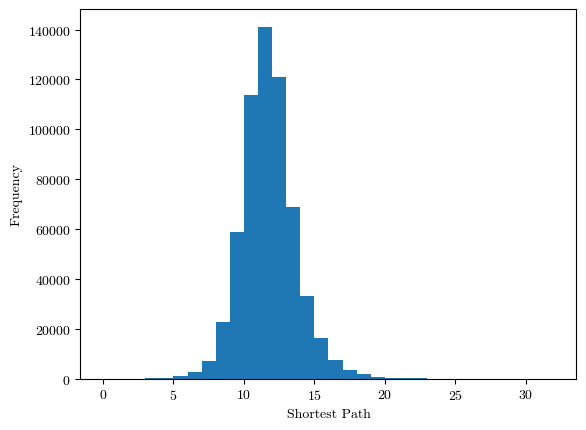
\includegraphics[width=0.5\textwidth]{shortest-paths-distribution.png}}
\caption{Shortest Paths Distribution Plot}
\label{sPathsPlot}
\end{figure}

\subsection{Triangle Count}

The total number of triangles in our graph was found to be 13391903. This is the same number of triangles as the one listed on the Triangle count value on the dataset statistics \cite{b5} \cite{b6}.

\subsection{Weakly Connected Components}

For the Weakly Connected Components, we first found the index of the largest WCC, which turned out to be equal to 0 and then we calculated the number of nodes in the largest WCC. That was found to be equal to 855802, which matches the value Nodes in largest WCC on the dataset statistics \cite{b5}.

\section{\textbf{Execution Runtimes Analysis}}\label{times}

The following section presents the procedure that we followed to report the execution times of the queries on our dataset, for both the libraries. We will also present the results of the execution times and perform some analysis on them.

\subsection{Timing Procedure}

To select a consistent way to time the execution of the queries for both libraries, we decided to use the \verb|time| command, which is a command-line utility for measuring the \verb|real|, \verb|user| and \verb|sys| CPU time of a program. The \verb|real| time is the total time that the program took to run from start to finish, the \verb|user| time is the time spent executing the program itself, outside of the kernel and the \verb|sys| time is the time spent in system calls within the kernel on behalf of the program. The \verb|time| command is available on most Unix-like operating systems, including \verb|Linux| and \verb|macOS|.

We examined a few other options for timing the execution of the queries, such as build in \verb|Listeners| on Spark, or \verb|Metric Reporters|, like \verb|Prometheus| on Flink. However, we could not vouch for the consistency of the results that they would provide, since we were not able to make sure that they were timing the similar parts of the code, meaning that one solution for one library might time just the execution of a job, while the other one also adds the time it takes to start the cluster and submit the job. So, we opted for the \verb|time| command as a more consistent and reliable way to time the whole execution of the queries.

The comparison will be based on the \verb|real| time and the sum \verb|user| and \verb|sys| times. The three metrics to be used are the average, minimum and maximum query execution time.

\subsection{Execution Times}

The execution times of the queries on our dataset, for both libraries, are presented in the following graphs, one for each query. In each of the graphs, there are 4 lines, one for GraphX \verb|real| time, one for GraphX \verb|user| and \verb|sys| time, and two more for Flink respectively. All times are in seconds.

\begin{figure}[htbp]
\centerline{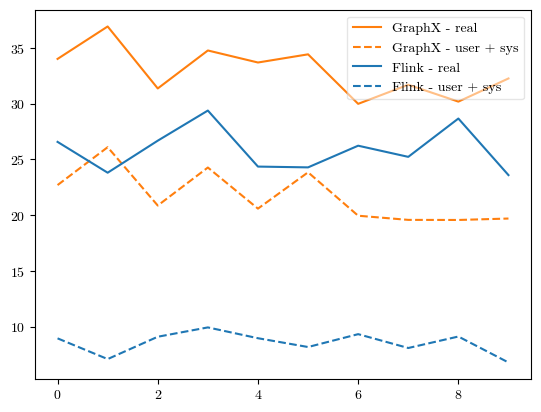
\includegraphics[width=0.5\textwidth]{degree-centrality-times.png}}
\caption{Degree Centrality Times}
\label{degreeTimes}
\end{figure}

\begin{figure}[htbp]
\centerline{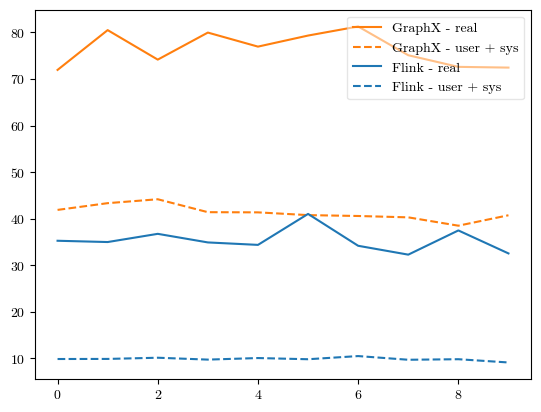
\includegraphics[width=0.5\textwidth]{shortest-paths-times.png}}
\caption{Shortest Path Times}
\label{shortestTimes}
\end{figure}

\begin{figure}[htbp]
\centerline{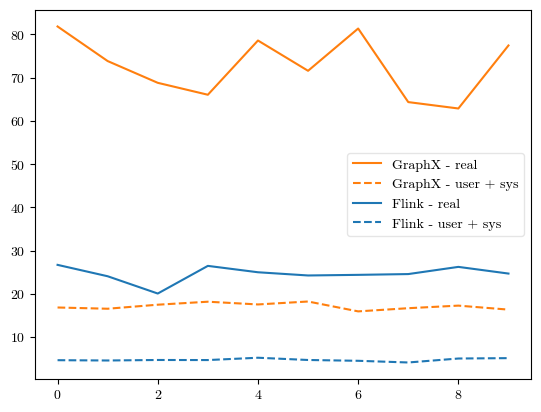
\includegraphics[width=0.5\textwidth]{triangle-count-times.png}}
\caption{Triangle Count Times}
\label{triangleTimes}
\end{figure}

\begin{figure}[htbp]
\centerline{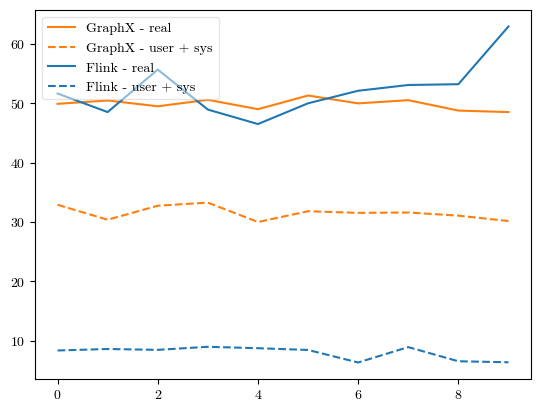
\includegraphics[width=0.5\textwidth]{weakly-connected-components-times.png}}
\caption{Weakly Connected Components Times}
\label{weaklyTimes}
\end{figure}

\subsection{Metrics}

The following section will showcase the average the minimum and the maximum query execution time for each query, for both libraries. These were calculated for both the \verb|real| time and the sum of \verb|user| and \verb|sys| times. The results are presented in the following six tables, the first one is the average \verb|real| time for both libraries per query. The second one is the minimum \verb|real| time again for both libraries per query. The third is the maximum \verb|real| time for both libraries per query. The fourth, fifth and sixth tables are the same as the first three but for the \verb|user+sys| time. The results are presented in the following tables.  

\begin{table}[htbp]
\caption{Average Query Time - Real}
\centering
\begin{tabular}{|c|c|c|}
\hline
\textbf{Query} & \textbf{GraphX} & \textbf{Flink}\\
\hline
Degree Centrality & 32.920 & 25.881 \\
\hline
Shortest Paths & 76.437 & 35.372 \\
\hline
Triangle Count & 72.660 & 24.639 \\
\hline
Weakly Connected Components & 49.861 & 52.266 \\
\hline
\end{tabular}
\end{table}

\begin{table}[htbp]
\caption{Minimum Query Time - Real}
\centering
\begin{tabular}{|c|c|c|}
\hline
\textbf{Query} & \textbf{GraphX} & \textbf{Flink}\\
\hline
Degree Centrality & 29.978 & 23.598 \\
\hline
Shortest Paths &71.957 & 32.272 \\
\hline
Triangle Count & 62.858 & 20.068 \\
\hline
Weakly Connected Components & 48.523 & 46.504 \\
\hline
\end{tabular}
\end{table}

\begin{table}[htbp]
\caption{Maximum Query Time - Real}
\centering
\begin{tabular}{|c|c|c|}
\hline
\textbf{Query} & \textbf{GraphX} & \textbf{Flink}\\
\hline
Degree Centrality & 36.905 & 29.377 \\
\hline
Shortest Paths & 81.287 & 41.021 \\
\hline
Triangle Count & 81.823 & 26.697 \\
\hline
Weakly Connected Components & 51.315 & 62.942 \\
\hline
\end{tabular}
\end{table}

\begin{table}[htbp]
\caption{Average Query Time - User+Sys}
\centering
\begin{tabular}{|c|c|c|}
\hline
\textbf{Query} & \textbf{GraphX} & \textbf{Flink}\\
\hline
Degree Centrality & 21.723 & 8.582 \\
\hline
Shortest Paths & 41.299 & 9.853 \\
\hline
Triangle Count & 17.106 & 4.734 \\
\hline
Weakly Connected Components & 31.552 & 7.980 \\
\hline
\end{tabular}
\end{table}

\begin{table}[htbp]
\caption{Minimum Query Time - User+Sys}
\centering
\begin{tabular}{|c|c|c|}
\hline
\textbf{Query} & \textbf{GraphX} & \textbf{Flink}\\
\hline
Degree Centrality & 19.580 & 6.820 \\
\hline
Shortest Paths & 38.492 & 9.108 \\
\hline
Triangle Count & 15.940 & 4.124 \\
\hline
Weakly Connected Components & 30.004 & 6.340 \\
\hline
\end{tabular}
\end{table}

\begin{table}[htbp]
\caption{Maximum Query Time - User+Sys}
\centering
\begin{tabular}{|c|c|c|}
\hline
\textbf{Query} & \textbf{GraphX} & \textbf{Flink}\\
\hline
Degree Centrality & 26.096 & 9.960 \\
\hline
Shortest Paths & 44.172 & 10.484 \\
\hline
Triangle Count & 18.224 & 5.220 \\
\hline
Weakly Connected Components & 33.272 & 8.984 \\
\hline
\end{tabular}
\end{table}

\subsection{Comparison}

First, we will examine the graphs containing the times for all the executions of the queries. 

\begin{itemize}
\item Degree Centrality Times: Flink maintains an advantage on \verb|real| time and is marginally better on \verb|user + sys| time. 

\item Shortest Paths Times: It is clear that Flink is much faster than GraphX, since even Flink's \verb|real| time is lower than GraphX's \verb|user+sys| time.

\item Triangle Count Times: Flink is once again noticeably faster than GraphX, nearly having faster \verb|real| time than GraphX's \verb|user+sys| time.

\item Weakly Connected Components Times: GraphX maintains a lower \verb|real| time through the majority of the runs, while Flink is consistently faster on \verb|user+sys| time.
\end{itemize}

Now, we will examine the average, minimum and maximum times for each query, for both libraries.

\begin{itemize}
\item \verb|real|: For the average query time, Flink is faster on Degree Centrality, and more than two times faster on Shortest Paths and Triangle Count. However, GraphX is slightly faster on Weakly Connected Components. 

\item \verb|real|: For minimum and maximum query time, Flink is faster on both and for all queries, especially for the Shortest Paths and Triangle Count. The only exception is for maximum query time on Weakly Connected Components, where GraphX is faster.

\item \verb|user+sys|: Flink is clearly faster on every metric (average, minimum and maximum query time) for all queries.
\end{itemize}


\section{\textbf{Conclusion}}\label{final}
In this section we discuss the results of our analysis and provide our conclusion.

\subsection{Results}

For the Degree Centrality query, which is a rather simple one, we see that Flink beats GraphX in a comfortable margin, both in terms of \verb|real| time and \verb|user+sys| time. There is a mention worthy difference in the \verb|user+sys| time, where Flink has a significant advantage, which points to the fact that Flink is using more efficient data structures and algorithms that require less CPU time in the \verb|user| and \verb|sys| modes. However, when \verb|real| time is considered, the difference is reduced but not eliminated.

For both the Shortest Paths and Triangle Count queries, it is clear that Flink is almost twice as fast as GraphX, both in terms of \verb|real| time and \verb|user+sys| time. So, in this case, Flink definitely utilizes faster algorithms and processes data more efficiently.

Finally, for the Weakly Connected Components, GraphX is slightly faster on \verb|real| time, but once again Flink wins with a noticeable difference in terms of \verb|user+sys| time. This is the only query where GraphX seems to be faster than Flink and that should be due to an efficient implementation of the algorithm and the data structures used by it. However, Flink's advantage in \verb|user+sys| times suggests it may still be more efficient overall, especially in a larger and more complex graph.

\subsection{Final Comments}

Based on the results presented in this paper, it can be concluded that Apache Flink outperforms Apache Spark GraphX in terms of query execution time for the majority of the graph processing queries tested. Specifically, Flink shows significant advantages in both \verb|real| and \verb|user+sys| time for the Degree Centrality, Shortest Paths, and Triangle Count queries. Although GraphX is slightly faster in \verb|real| time for the Weakly Connected Components query, Flink's advantage in \verb|user+sys| time suggests that it may still be a more efficient choice, in the cases of a more complex graph processing tasks. 

Overall, this paper provides valuable insights into the performance differences between these two popular graph processing systems, which can aid in the selection and optimization of graph processing solutions for various applications.

\begin{thebibliography}{00}
\bibitem{b1} “GraphX: Apache Spark,” GraphX | Apache Spark. [Online]. Available: https://spark.apache.org/graphx/.
\bibitem{b2} “Apache Flink® - stateful computations over data streams,” Apache Flink® - Stateful Computations over Data Streams | Apache Flink. [Online]. Available: https://flink.apache.org/.
\bibitem{b3} G. Kyriakopoulos, “geokyr/ntua-information-systems: Apache Spark GraphX and Apache Flink project for the Analysis and Design of Information Systems course at ECE NTUA,” GitHub. [Online]. Available: https://github.com/geokyr/ntua-information-systems. 
\bibitem{b4} S. Tzelepis, “Sertze/InformationSystems: Analysis and Design of Information Systems,” GitHub. [Online]. Available: https://github.com/SerTze/InformationSystems.
\bibitem{b5} “Google Web Graph,” SNAP. [Online]. Available: https://snap.stanford.edu/data/web-Google.html.
\bibitem{b6} “Google Hyperlinks,” Google hyperlinks. [Online]. Available: http://konect.cc/networks/web-Google/.
\bibitem{b7} “~Okeanos,” ~okeanos Dashboard. [Online]. Available: https://accounts.okeanos.grnet.gr/.
\bibitem{b8} “Download the latest Java Lts Free,” Oracle. [Online]. Available: https://www.oracle.com/java/technologies/downloads/. 
\bibitem{b9} “Apache spark™ - unified engine for large-scale data analytics,” Apache Spark™ - Unified Engine for large-scale data analytics. [Online]. Available: https://spark.apache.org/.
\bibitem{b10} “The Scala programming language,” News. [Online]. Available: https://www.scala-lang.org/.
\bibitem{b11} “The Interactive Build Tool,” sbt. [Online]. Available: https://www.scala-sbt.org/.
\bibitem{b12} B. Porter, J. van Zyl, and O. Lamy, “Welcome to Apache Maven,” Maven. [Online]. Available: https://maven.apache.org/. 
\bibitem{b13} “Project jupyter,” Project Jupyter. [Online]. Available: https://jupyter.org/.
\bibitem{b14} Google colab. [Online]. Available: https://colab.research.google.com/.
\bibitem{b15} “Pandas,” pandas. [Online]. Available: https://pandas.pydata.org/.
\end{thebibliography}

\end{document}